\documentclass[12pt,a4paper]{article}

\usepackage[a4paper,text={16.5cm,25.2cm},centering]{geometry}
\usepackage{lmodern}
\usepackage{amssymb,amsmath}
\usepackage{bm}
\usepackage{graphicx}
\usepackage{microtype}
\usepackage{hyperref}
\setlength{\parindent}{0pt}
\setlength{\parskip}{1.2ex}

\hypersetup
       {   pdfauthor = { Marco Fasondini },
           pdftitle={ foo },
           colorlinks=TRUE,
           linkcolor=black,
           citecolor=blue,
           urlcolor=blue
       }




\usepackage{upquote}
\usepackage{listings}
\usepackage{xcolor}
\lstset{
    basicstyle=\ttfamily\footnotesize,
    upquote=true,
    breaklines=true,
    breakindent=0pt,
    keepspaces=true,
    showspaces=false,
    columns=fullflexible,
    showtabs=false,
    showstringspaces=false,
    escapeinside={(*@}{@*)},
    extendedchars=true,
}
\newcommand{\HLJLt}[1]{#1}
\newcommand{\HLJLw}[1]{#1}
\newcommand{\HLJLe}[1]{#1}
\newcommand{\HLJLeB}[1]{#1}
\newcommand{\HLJLo}[1]{#1}
\newcommand{\HLJLk}[1]{\textcolor[RGB]{148,91,176}{\textbf{#1}}}
\newcommand{\HLJLkc}[1]{\textcolor[RGB]{59,151,46}{\textit{#1}}}
\newcommand{\HLJLkd}[1]{\textcolor[RGB]{214,102,97}{\textit{#1}}}
\newcommand{\HLJLkn}[1]{\textcolor[RGB]{148,91,176}{\textbf{#1}}}
\newcommand{\HLJLkp}[1]{\textcolor[RGB]{148,91,176}{\textbf{#1}}}
\newcommand{\HLJLkr}[1]{\textcolor[RGB]{148,91,176}{\textbf{#1}}}
\newcommand{\HLJLkt}[1]{\textcolor[RGB]{148,91,176}{\textbf{#1}}}
\newcommand{\HLJLn}[1]{#1}
\newcommand{\HLJLna}[1]{#1}
\newcommand{\HLJLnb}[1]{#1}
\newcommand{\HLJLnbp}[1]{#1}
\newcommand{\HLJLnc}[1]{#1}
\newcommand{\HLJLncB}[1]{#1}
\newcommand{\HLJLnd}[1]{\textcolor[RGB]{214,102,97}{#1}}
\newcommand{\HLJLne}[1]{#1}
\newcommand{\HLJLneB}[1]{#1}
\newcommand{\HLJLnf}[1]{\textcolor[RGB]{66,102,213}{#1}}
\newcommand{\HLJLnfm}[1]{\textcolor[RGB]{66,102,213}{#1}}
\newcommand{\HLJLnp}[1]{#1}
\newcommand{\HLJLnl}[1]{#1}
\newcommand{\HLJLnn}[1]{#1}
\newcommand{\HLJLno}[1]{#1}
\newcommand{\HLJLnt}[1]{#1}
\newcommand{\HLJLnv}[1]{#1}
\newcommand{\HLJLnvc}[1]{#1}
\newcommand{\HLJLnvg}[1]{#1}
\newcommand{\HLJLnvi}[1]{#1}
\newcommand{\HLJLnvm}[1]{#1}
\newcommand{\HLJLl}[1]{#1}
\newcommand{\HLJLld}[1]{\textcolor[RGB]{148,91,176}{\textit{#1}}}
\newcommand{\HLJLs}[1]{\textcolor[RGB]{201,61,57}{#1}}
\newcommand{\HLJLsa}[1]{\textcolor[RGB]{201,61,57}{#1}}
\newcommand{\HLJLsb}[1]{\textcolor[RGB]{201,61,57}{#1}}
\newcommand{\HLJLsc}[1]{\textcolor[RGB]{201,61,57}{#1}}
\newcommand{\HLJLsd}[1]{\textcolor[RGB]{201,61,57}{#1}}
\newcommand{\HLJLsdB}[1]{\textcolor[RGB]{201,61,57}{#1}}
\newcommand{\HLJLsdC}[1]{\textcolor[RGB]{201,61,57}{#1}}
\newcommand{\HLJLse}[1]{\textcolor[RGB]{59,151,46}{#1}}
\newcommand{\HLJLsh}[1]{\textcolor[RGB]{201,61,57}{#1}}
\newcommand{\HLJLsi}[1]{#1}
\newcommand{\HLJLso}[1]{\textcolor[RGB]{201,61,57}{#1}}
\newcommand{\HLJLsr}[1]{\textcolor[RGB]{201,61,57}{#1}}
\newcommand{\HLJLss}[1]{\textcolor[RGB]{201,61,57}{#1}}
\newcommand{\HLJLssB}[1]{\textcolor[RGB]{201,61,57}{#1}}
\newcommand{\HLJLnB}[1]{\textcolor[RGB]{59,151,46}{#1}}
\newcommand{\HLJLnbB}[1]{\textcolor[RGB]{59,151,46}{#1}}
\newcommand{\HLJLnfB}[1]{\textcolor[RGB]{59,151,46}{#1}}
\newcommand{\HLJLnh}[1]{\textcolor[RGB]{59,151,46}{#1}}
\newcommand{\HLJLni}[1]{\textcolor[RGB]{59,151,46}{#1}}
\newcommand{\HLJLnil}[1]{\textcolor[RGB]{59,151,46}{#1}}
\newcommand{\HLJLnoB}[1]{\textcolor[RGB]{59,151,46}{#1}}
\newcommand{\HLJLoB}[1]{\textcolor[RGB]{102,102,102}{\textbf{#1}}}
\newcommand{\HLJLow}[1]{\textcolor[RGB]{102,102,102}{\textbf{#1}}}
\newcommand{\HLJLp}[1]{#1}
\newcommand{\HLJLc}[1]{\textcolor[RGB]{153,153,119}{\textit{#1}}}
\newcommand{\HLJLch}[1]{\textcolor[RGB]{153,153,119}{\textit{#1}}}
\newcommand{\HLJLcm}[1]{\textcolor[RGB]{153,153,119}{\textit{#1}}}
\newcommand{\HLJLcp}[1]{\textcolor[RGB]{153,153,119}{\textit{#1}}}
\newcommand{\HLJLcpB}[1]{\textcolor[RGB]{153,153,119}{\textit{#1}}}
\newcommand{\HLJLcs}[1]{\textcolor[RGB]{153,153,119}{\textit{#1}}}
\newcommand{\HLJLcsB}[1]{\textcolor[RGB]{153,153,119}{\textit{#1}}}
\newcommand{\HLJLg}[1]{#1}
\newcommand{\HLJLgd}[1]{#1}
\newcommand{\HLJLge}[1]{#1}
\newcommand{\HLJLgeB}[1]{#1}
\newcommand{\HLJLgh}[1]{#1}
\newcommand{\HLJLgi}[1]{#1}
\newcommand{\HLJLgo}[1]{#1}
\newcommand{\HLJLgp}[1]{#1}
\newcommand{\HLJLgs}[1]{#1}
\newcommand{\HLJLgsB}[1]{#1}
\newcommand{\HLJLgt}[1]{#1}



\def\qqand{\qquad\hbox{and}\qquad}
\def\qqfor{\qquad\hbox{for}\qquad}
\def\qqas{\qquad\hbox{as}\qquad}
\def\half{ {1 \over 2} }
\def\D{ {\rm d} }
\def\I{ {\rm i} }
\def\E{ {\rm e} }
\def\C{ {\mathbb C} }
\def\R{ {\mathbb R} }
\def\bbR{ {\mathbb R} }
\def\H{ {\mathbb H} }
\def\Z{ {\mathbb Z} }
\def\CC{ {\cal C} }
\def\FF{ {\cal F} }
\def\HH{ {\cal H} }
\def\LL{ {\cal L} }
\def\vc#1{ {\mathbf #1} }
\def\bbC{ {\mathbb C} }



\def\fR{ f_{\rm R} }
\def\fL{ f_{\rm L} }

\def\qqqquad{\qquad\qquad}
\def\qqwhere{\qquad\hbox{where}\qquad}
\def\Res_#1{\underset{#1}{\rm Res}\,}
\def\sech{ {\rm sech}\, }
\def\acos{ {\rm acos}\, }
\def\asin{ {\rm asin}\, }
\def\atan{ {\rm atan}\, }
\def\Ei{ {\rm Ei}\, }
\def\upepsilon{\varepsilon}


\def\Xint#1{ \mathchoice
   {\XXint\displaystyle\textstyle{#1} }%
   {\XXint\textstyle\scriptstyle{#1} }%
   {\XXint\scriptstyle\scriptscriptstyle{#1} }%
   {\XXint\scriptscriptstyle\scriptscriptstyle{#1} }%
   \!\int}
\def\XXint#1#2#3{ {\setbox0=\hbox{$#1{#2#3}{\int}$}
     \vcenter{\hbox{$#2#3$}}\kern-.5\wd0} }
\def\ddashint{\Xint=}
\def\dashint{\Xint-}
% \def\dashint
\def\infdashint{\dashint_{-\infty}^\infty}




\def\addtab#1={#1\;&=}
\def\ccr{\\\addtab}
\def\ip<#1>{\left\langle{#1}\right\rangle}
\def\dx{\D x}
\def\dt{\D t}
\def\dz{\D z}
\def\ds{\D s}

\def\rR{ {\rm R} }
\def\rL{ {\rm L} }

\def\norm#1{\left\| #1 \right\|}

\def\pr(#1){\left({#1}\right)}
\def\br[#1]{\left[{#1}\right]}

\def\abs#1{\left|{#1}\right|}
\def\fpr(#1){\!\pr({#1})}

\def\sopmatrix#1{ \begin{pmatrix}#1\end{pmatrix} }

\def\endash{–}
\def\emdash{—}
\def\mdblksquare{\blacksquare}
\def\lgblksquare{\blacksquare}
\def\scre{\E}
\def\mapengine#1,#2.{\mapfunction{#1}\ifx\void#2\else\mapengine #2.\fi }

\def\map[#1]{\mapengine #1,\void.}

\def\mapenginesep_#1#2,#3.{\mapfunction{#2}\ifx\void#3\else#1\mapengine #3.\fi }

\def\mapsep_#1[#2]{\mapenginesep_{#1}#2,\void.}


\def\vcbr[#1]{\pr(#1)}


\def\bvect[#1,#2]{
{
\def\dots{\cdots}
\def\mapfunction##1{\ | \  ##1}
	\sopmatrix{
		 \,#1\map[#2]\,
	}
}
}



\def\vect[#1]{
{\def\dots{\ldots}
	\vcbr[{#1}]
} }

\def\vectt[#1]{
{\def\dots{\ldots}
	\vect[{#1}]^{\top}
} }

\def\Vectt[#1]{
{
\def\mapfunction##1{##1 \cr}
\def\dots{\vdots}
	\begin{pmatrix}
		\map[#1]
	\end{pmatrix}
} }

\def\addtab#1={#1\;&=}
\def\ccr{\\\addtab}

\def\questionequals{= \!\!\!\!\!\!{\scriptstyle ? \atop }\,\,\,}

\def\Ei{\rm Ei\,}

\begin{document}

\section{Problem sheet 2: Solutions}
The (well-posed) convection-diffusion equation is 

\[
\frac{\partial u}{\partial t} = \frac{\partial^2 u}{\partial x^2} - b \frac{\partial u}{\partial x}, \qquad 0 \leq x \leq 1, \: 0 \leq t \leq T, T > 0,
\]
where $b > 0$ is given (a constant) and the boundary conditions are $u(0,t) = \varphi_0(t)$ and $u(1,t) = \varphi_1(t)$ for $t \in [0, T]$.  Let 

\[
v'_j = \frac{1}{h^2}\left(v_{j-1} - 2v_j + v_{j+1}   \right) - \frac{b}{2h}\left(v_{j+1}  - v_{j-1}   \right), \qquad j =  1, 2,  \ldots, n_x,
\]
where $h = \displaystyle{\frac{1}{n_x + 1}}$ and $v_j = v_j(t)$ be a semi-discrete method for the convection-diffusion equation.

\begin{itemize}
\item[1. ] \textbf{[5 marks]} Prove that the semi-discrete method is second-order accurate.  That is, let $\widetilde{v}_j(t) =  u(x_j,t)$ and show that (assuming all the relevant partial derivatives are bounded on $(x,t) \in [0, 1]\times [0, T]$),

\end{itemize}
\[
\widetilde{v}'_j - \frac{1}{h^2}\left(\widetilde{v}_{j-1} - 2\widetilde{v}_j + \widetilde{v}_{j+1}   \right) + \frac{b}{2h}\left(\widetilde{v}_{j+1}  - \widetilde{v}_{j-1}   \right) = \mathcal{O}\left(h^2 \right), \qquad h \to 0.
\]
\textbf{Solution}  Using Taylor's theorem (see Chapter 1), there exists a $\xi_+ \in (x_j, x_j + h)$  such that


\begin{eqnarray*}
\widetilde{v}_{j + 1} &=& u(x_{j+1},t) \\
&=&u(x_j + h,t) \\
&=& u(x_j,t) +  hu_x(x_j,t) + \frac{h^2}{2}u_{xx}(x_j,t) + \frac{h^3}{6}u_{xxx}(x_j,t) + \frac{h^4}{24}u_{xxxx} (\xi_+,t) \\
&=& \widetilde{v}_{j} +  hu_x(x_j,t) + \frac{h^2}{2}u_{xx}(x_j,t) + \frac{h^3}{6}u_{xxx}(x_j,t) + \frac{h^4}{24}u_{xxxx} (\xi_+,t).
\end{eqnarray*}
Similarly, by replacing $h$ with $-h$ in the equations above,  there exists a $\xi_- \in (x_j - h, x_j)$  such that


\begin{eqnarray*}
\widetilde{v}_{j - 1} &=& u(x_{j-1},t) \\
&=&u(x_j - h,t) \\
&=& u(x_j,t) -  hu_x(x_j,t) + \frac{h^2}{2}u_{xx}(x_j,t) - \frac{h^3}{6}u_{xxx}(x_j,t) + \frac{h^4}{24}u_{xxxx} (\xi_-,t) \\
&=& \widetilde{v}_{j} -  hu_x(x_j,t) + \frac{h^2}{2}u_{xx}(x_j,t) - \frac{h^3}{6}u_{xxx}(x_j,t) + \frac{h^4}{24}u_{xxxx} (\xi_-,t).
\end{eqnarray*}
Hence, it follows that


\begin{equation*}
\frac{1}{h^2}\left(\widetilde{v}_{j-1} - 2\widetilde{v}_j + \widetilde{v}_{j+1}   \right) = u_{xx}(x_j,t) + \frac{h^2}{24}\left(u_{xxxx} (\xi_+,t) + u_{xxxx} (\xi_-,t)  \right)
\end{equation*}
and we conclude that (since we assume that $u_{xxxx}$ is bounded)


\begin{equation}
\frac{1}{h^2}\left(\widetilde{v}_{j-1} - 2\widetilde{v}_j + \widetilde{v}_{j+1}   \right) = u_{xx}(x_j,t) + \mathcal{O}\left(h^2\right), \qquad h \to 0. \qquad (\star)
\end{equation}
Also, it follows that


\begin{equation*}
\frac{1}{2h}\left(\widetilde{v}_{j+1} - \widetilde{v}_{j-1}   \right) = u_{x}(x_j,t) + \frac{h^2}{6}u_{xxx} (x_j,t) + \frac{h^3}{48}\left(u_{xxxx} (\xi_+,t) - u_{xxxx} (\xi_-,t)  \right)
\end{equation*}
and we conclude that (since we assume that $u_{xxx}$ and $u_{xxxx}$ are bounded)


\begin{equation}
\frac{1}{2h}\left(\widetilde{v}_{j+1} - \widetilde{v}_{j-1}   \right) = u_{x}(x_j,t) + \mathcal{O}\left(h^2\right), \qquad h \to 0. \qquad (\diamond)
\end{equation}
Using $(\star)$ and $(\diamond)$ and the advection-diffusion equation, it follows that as $h \to 0$,


\begin{eqnarray*}
&& \widetilde{v}'_j - \frac{1}{h^2}\left(\widetilde{v}_{j-1} - 2\widetilde{v}_j + \widetilde{v}_{j+1}   \right) + \frac{b}{2h}\left(\widetilde{v}_{j+1}  - \widetilde{v}_{j-1}   \right) \\
&& = \underbrace{u_t(x_j,t) - u_{xx}(x_j,t) + bu_{x}(x_j,t)}_{=\: 0} +  \mathcal{O}\left(h^2\right) \\
&& = \mathcal{O}\left(h^2\right).
\end{eqnarray*}
\begin{itemize}
\item[2. ] \textbf{[2 marks]} Is the semi-discrete method consistent?  Motivate your answer.

\textbf{Solution} Yes, since the method is second-order, the local error tends to zero as $h \to 0$ and therefore the method is consistent.


\item[3. ] \textbf{[6 marks]} Use the von Neumann method to determine whether the semi-discrete method is stable.

\textbf{Solution} 

\end{itemize}
Substituting

\[
v_j(t) = v_j = \lambda(t)\mathrm{e}^{{\mathrm{i}}kx_j} = \lambda \mathrm{e}^{{\mathrm{i}}kx_j},
\]
where $x_j = jh$ and $k \in \mathbb{Z}$, into the semi-discrete method and using the fact that $v_{j+1} = \lambda \mathrm{e}^{{\mathrm{i}}kx_{j+1}} = \lambda \mathrm{e}^{{\mathrm{i}}k(x_{j}+h)} = \mathrm{e}^{{\mathrm{i}}kh}v_j$, we find that


\begin{eqnarray*}
v_j' &=& \frac{1}{h^2}\left(\mathrm{e}^{{-\mathrm{i}}kh} - 2 + \mathrm{e}^{{\mathrm{i}}kh}   \right)v_j - \frac{b}{2h}\left(\mathrm{e}^{{\mathrm{i}}kh}  - \mathrm{e}^{-{\mathrm{i}}kh}   \right)v_j \\
&=& \frac{1}{h^2}\left(2\cos(kh) - 2   \right)v_j - \frac{b}{2h}\left( 2\mathrm{i}\sin(kh)   \right)v_j \\
&=& -\frac{2}{h^2}\left(1 - \cos(kh)   \right)v_j - \frac{b\mathrm{i}}{h} \sin(kh)  v_j \\
&=& -\left[\frac{4}{h^2}\sin^2(kh/2) + \frac{b\mathrm{i}}{h} \sin(kh)\right]  v_j \\
& \Longrightarrow & \lambda' = -\left[\frac{4}{h^2}\sin^2(kh/2) + \frac{b\mathrm{i}}{h} \sin(kh)\right] \lambda \\
& \Longrightarrow & \lambda(t) = \exp\left( -\left[\frac{4}{h^2}\sin^2(kh/2) + \frac{b\mathrm{i}}{h} \sin(kh)\right] t  \right)\lambda(0).
\end{eqnarray*}
Since, as $h \to 0$,


\begin{equation*}
\frac{4}{h^2}\sin^2(kh/2) = k^2 + \mathcal{O}\left(h^2\right), \qquad \frac{1}{h} \sin(kh) = k + \mathcal{O}\left(h^2\right),
\end{equation*}
we have that for $t \in [0, T]$,


\begin{eqnarray*}
\lim_{h \to 0}\left\vert  \lambda(t)  \right\vert &=& \lim_{h \to 0}\left\vert  \exp\left( -\left[\frac{4}{h^2}\sin^2(kh/2) + \frac{b\mathrm{i}}{h} \sin(kh)\right] t  \right)\lambda(0)  \right\vert \\
&=& \lim_{h \to 0}  \exp\left( -\frac{4}{h^2}\sin^2(kh/2) t  \right)\left\vert\lambda(0)  \right\vert \\
&=& \mathrm{e}^{-k^2t}\left\vert\lambda(0)  \right\vert\\
& \leq & \left\vert\lambda(0)  \right\vert \\
& < & \infty
\end{eqnarray*}
hence the method is stable.

\begin{itemize}
\item[4. ] \textbf{[2 marks]} Is the semi-discrete method convergent?

\textbf{Solution} Yes, since the advection-diffusion equation is well-posed and the semi-discrete method is consistent and stable, it is convergent by the Lax equivalence theorem.


\item[5. ] \textbf{[5 marks]} Show that the semi-discrete method can be expressed as the following system of ordinary differential equations (ODEs):

\end{itemize}
\[
\mathbf{v}' = A\mathbf{v} + \mathbf{h}
\]
with $\mathbf{v}, \mathbf{h} \in \mathbb{R}^{n_x}$, $A \in \mathbb{R}^{n_x \times n_x}$ where

\[
A = \frac{1}{h^2}\begin{bmatrix}
-2 & 1 - \frac{bh}{2} & & & \\
1 + \frac{bh}{2}  & -2 & 1 - \frac{bh}{2}  & & \\
      & \ddots & \ddots & \ddots & \\
      &        & 1 + \frac{bh}{2}    & -2 & 1 - \frac{bh}{2} \\
      &        &        &1 + \frac{bh}{2}      & -2
\end{bmatrix}, \quad
\mathbf{h} = \frac{1}{h^2}\left[\begin{array}{c} 
{} \left(1 + \frac{bh}{2}\right)\varphi_0(t)\\
0 \\
\vdots \\
0 \\
\left(1 - \frac{bh}{2}\right)\varphi_1(t)
\end{array}
\right]
\]
\textbf{Solution} Rewriting the semi-discrete method


\begin{eqnarray*}
v'_j &=& \frac{1}{h^2}\left(v_{j-1} - 2v_j + v_{j+1}   \right) - \frac{b}{2h}\left(v_{j+1}  - v_{j-1}   \right) \\
&=& \frac{1}{h^2}\left[ \left(1 + \frac{bh}{2}\right)v_{j-1} - 2v_j +  \left(1 - \frac{bh}{2}\right)v_{j+1}  \right],\qquad j = 1, \ldots, n_x,
\end{eqnarray*}
it follows that


\begin{equation*}
\mathbf{v}' = A\mathbf{v} + \mathbf{h}
\end{equation*}
where


\begin{equation*}
\mathbf{v} = \left(\begin{array}{c}
v_1\\
v_2 \\
\vdots \\
v_{n_x}
\end{array}
\right), \quad A = \frac{1}{h^2}\begin{bmatrix}
-2 & 1 - \frac{bh}{2} & & & \\
1 + \frac{bh}{2}  & -2 & 1 - \frac{bh}{2}  & & \\
      & \ddots & \ddots & \ddots & \\
      &        & 1 + \frac{bh}{2}    & -2 & 1 - \frac{bh}{2} \\
      &        &        &1 + \frac{bh}{2}      & -2
\end{bmatrix}, \quad
\mathbf{h} = \frac{1}{h^2}\left(\begin{array}{c} 
\left(1 + \frac{bh}{2}\right)\varphi_0(t)\\
0 \\
\vdots \\
0 \\
\left(1 - \frac{bh}{2}\right)\varphi_1(t)
\end{array}
\right)
\end{equation*}
\begin{itemize}
\item[6. ] \textbf{[10 marks]} Let $n_x = 300$, $T = 0.003$, $b = 100$, $\varphi_0(t) = 0 = \varphi_1(t)$ and $u(x,0) = \mathrm{e}^{-300(x-0.3)^2}$, then solve the ODE system in question 5 with an error tolerance of $10^{-4}$ using any ODE solver that's available in your programming language of choice.  Plot the solution at $t = 0$ and $t = T$ on the same set of axes.

\textbf{Solution}

\end{itemize}

\begin{lstlisting}
(*@\HLJLk{using}@*) (*@\HLJLn{LinearAlgebra}@*)(*@\HLJLp{,}@*) (*@\HLJLn{Plots}@*)(*@\HLJLp{,}@*) (*@\HLJLn{OrdinaryDiffEq}@*)

(*@\HLJLn{nx}@*) (*@\HLJLoB{=}@*) (*@\HLJLni{300}@*)
(*@\HLJLn{x}@*) (*@\HLJLoB{=}@*) (*@\HLJLnf{range}@*)(*@\HLJLp{(}@*)(*@\HLJLni{0}@*)(*@\HLJLp{,}@*)(*@\HLJLni{1}@*)(*@\HLJLp{,}@*)(*@\HLJLn{nx}@*)(*@\HLJLoB{+}@*)(*@\HLJLni{2}@*)(*@\HLJLp{)}@*)
(*@\HLJLn{f}@*) (*@\HLJLoB{=}@*) (*@\HLJLn{x}@*) (*@\HLJLoB{->}@*) (*@\HLJLnf{exp}@*)(*@\HLJLp{(}@*)(*@\HLJLoB{-}@*)(*@\HLJLni{300}@*)(*@\HLJLoB{*}@*)(*@\HLJLp{(}@*)(*@\HLJLn{x}@*)(*@\HLJLoB{-}@*)(*@\HLJLnfB{0.3}@*)(*@\HLJLp{)}@*)(*@\HLJLoB{.{\textasciicircum}}@*)(*@\HLJLni{2}@*)(*@\HLJLp{)}@*)
(*@\HLJLn{h}@*) (*@\HLJLoB{=}@*) (*@\HLJLni{1}@*)(*@\HLJLoB{/}@*)(*@\HLJLp{(}@*)(*@\HLJLn{nx}@*)(*@\HLJLoB{+}@*)(*@\HLJLni{1}@*)(*@\HLJLp{)}@*)
(*@\HLJLn{T}@*) (*@\HLJLoB{=}@*) (*@\HLJLnfB{0.003}@*)
(*@\HLJLn{b}@*) (*@\HLJLoB{=}@*) (*@\HLJLni{100}@*)
(*@\HLJLn{A}@*) (*@\HLJLoB{=}@*) (*@\HLJLnf{Tridiagonal}@*)(*@\HLJLp{(}@*)(*@\HLJLnf{fill}@*)(*@\HLJLp{(}@*)(*@\HLJLni{1}@*)(*@\HLJLoB{+}@*)(*@\HLJLn{b}@*)(*@\HLJLoB{*}@*)(*@\HLJLn{h}@*)(*@\HLJLoB{/}@*)(*@\HLJLni{2}@*)(*@\HLJLp{,}@*)(*@\HLJLn{nx}@*)(*@\HLJLoB{-}@*)(*@\HLJLni{1}@*)(*@\HLJLp{),}@*)(*@\HLJLnf{fill}@*)(*@\HLJLp{(}@*)(*@\HLJLoB{-}@*)(*@\HLJLnfB{2.0}@*)(*@\HLJLp{,}@*)(*@\HLJLn{nx}@*)(*@\HLJLp{),}@*)(*@\HLJLnf{fill}@*)(*@\HLJLp{(}@*)(*@\HLJLni{1}@*)(*@\HLJLoB{-}@*)(*@\HLJLn{b}@*)(*@\HLJLoB{*}@*)(*@\HLJLn{h}@*)(*@\HLJLoB{/}@*)(*@\HLJLni{2}@*)(*@\HLJLp{,}@*)(*@\HLJLn{nx}@*)(*@\HLJLoB{-}@*)(*@\HLJLni{1}@*)(*@\HLJLp{))}@*)(*@\HLJLoB{/}@*)(*@\HLJLn{h}@*)(*@\HLJLoB{{\textasciicircum}}@*)(*@\HLJLni{2}@*)
(*@\HLJLn{F}@*) (*@\HLJLoB{=}@*) (*@\HLJLp{(}@*)(*@\HLJLn{v}@*)(*@\HLJLp{,}@*)(*@\HLJLn{p}@*)(*@\HLJLp{,}@*)(*@\HLJLn{t}@*)(*@\HLJLp{)}@*) (*@\HLJLoB{->}@*) (*@\HLJLn{A}@*)(*@\HLJLoB{*}@*)(*@\HLJLn{v}@*)
(*@\HLJLn{x}@*) (*@\HLJLoB{=}@*) (*@\HLJLnf{range}@*)(*@\HLJLp{(}@*)(*@\HLJLni{0}@*)(*@\HLJLp{,}@*)(*@\HLJLni{1}@*)(*@\HLJLp{,}@*)(*@\HLJLn{nx}@*) (*@\HLJLoB{+}@*) (*@\HLJLni{2}@*)(*@\HLJLp{)}@*)
(*@\HLJLn{prob}@*) (*@\HLJLoB{=}@*) (*@\HLJLnf{ODEProblem}@*)(*@\HLJLp{(}@*)(*@\HLJLn{F}@*)(*@\HLJLp{,}@*) (*@\HLJLn{f}@*)(*@\HLJLoB{.}@*)(*@\HLJLp{(}@*)(*@\HLJLn{x}@*)(*@\HLJLp{[}@*)(*@\HLJLni{2}@*)(*@\HLJLoB{:}@*)(*@\HLJLk{end}@*)(*@\HLJLoB{-}@*)(*@\HLJLni{1}@*)(*@\HLJLp{]),}@*) (*@\HLJLp{(}@*)(*@\HLJLnfB{0.0}@*)(*@\HLJLp{,}@*) (*@\HLJLn{T}@*)(*@\HLJLp{))}@*)
(*@\HLJLcs{{\#}soln}@*) (*@\HLJLcs{=}@*)  (*@\HLJLcs{solve(prob,}@*) (*@\HLJLcs{RK4(),abstol=1e-4)}@*)
(*@\HLJLcs{{\#}soln}@*) (*@\HLJLcs{=}@*)  (*@\HLJLcs{solve(prob,}@*) (*@\HLJLcs{Rodas4(),abstol=1e-4);}@*)
(*@\HLJLn{soln}@*) (*@\HLJLoB{=}@*)  (*@\HLJLnf{solve}@*)(*@\HLJLp{(}@*)(*@\HLJLn{prob}@*)(*@\HLJLp{,}@*) (*@\HLJLnf{Rodas4P}@*)(*@\HLJLp{(),}@*)(*@\HLJLn{abstol}@*)(*@\HLJLoB{=}@*)(*@\HLJLnfB{1e-4}@*)(*@\HLJLp{)}@*)
(*@\HLJLnd{@show}@*) (*@\HLJLn{nt}@*) (*@\HLJLoB{=}@*) (*@\HLJLnf{length}@*)(*@\HLJLp{(}@*)(*@\HLJLn{soln}@*)(*@\HLJLoB{.}@*)(*@\HLJLn{t}@*)(*@\HLJLp{)}@*)
(*@\HLJLnf{plot}@*)(*@\HLJLp{(}@*)(*@\HLJLn{x}@*)(*@\HLJLp{[}@*)(*@\HLJLni{2}@*)(*@\HLJLoB{:}@*)(*@\HLJLn{nx}@*)(*@\HLJLoB{+}@*)(*@\HLJLni{1}@*)(*@\HLJLp{],}@*)(*@\HLJLn{soln}@*)(*@\HLJLoB{.}@*)(*@\HLJLn{u}@*)(*@\HLJLp{[}@*)(*@\HLJLn{nt}@*)(*@\HLJLp{],}@*)(*@\HLJLn{label}@*) (*@\HLJLoB{=}@*) (*@\HLJLs{"{}t}@*) (*@\HLJLs{=}@*) (*@\HLJLs{0.003"{}}@*)(*@\HLJLp{)}@*)
(*@\HLJLnf{plot!}@*)(*@\HLJLp{(}@*)(*@\HLJLn{x}@*)(*@\HLJLp{[}@*)(*@\HLJLni{2}@*)(*@\HLJLoB{:}@*)(*@\HLJLn{nx}@*)(*@\HLJLoB{+}@*)(*@\HLJLni{1}@*)(*@\HLJLp{],}@*)(*@\HLJLn{soln}@*)(*@\HLJLoB{.}@*)(*@\HLJLn{u}@*)(*@\HLJLp{[}@*)(*@\HLJLni{1}@*)(*@\HLJLp{],}@*)(*@\HLJLn{label}@*) (*@\HLJLoB{=}@*) (*@\HLJLs{"{}t}@*) (*@\HLJLs{=}@*) (*@\HLJLs{0"{}}@*)(*@\HLJLp{)}@*)
\end{lstlisting}

\begin{lstlisting}
nt = length(soln.t) = 14
\end{lstlisting}

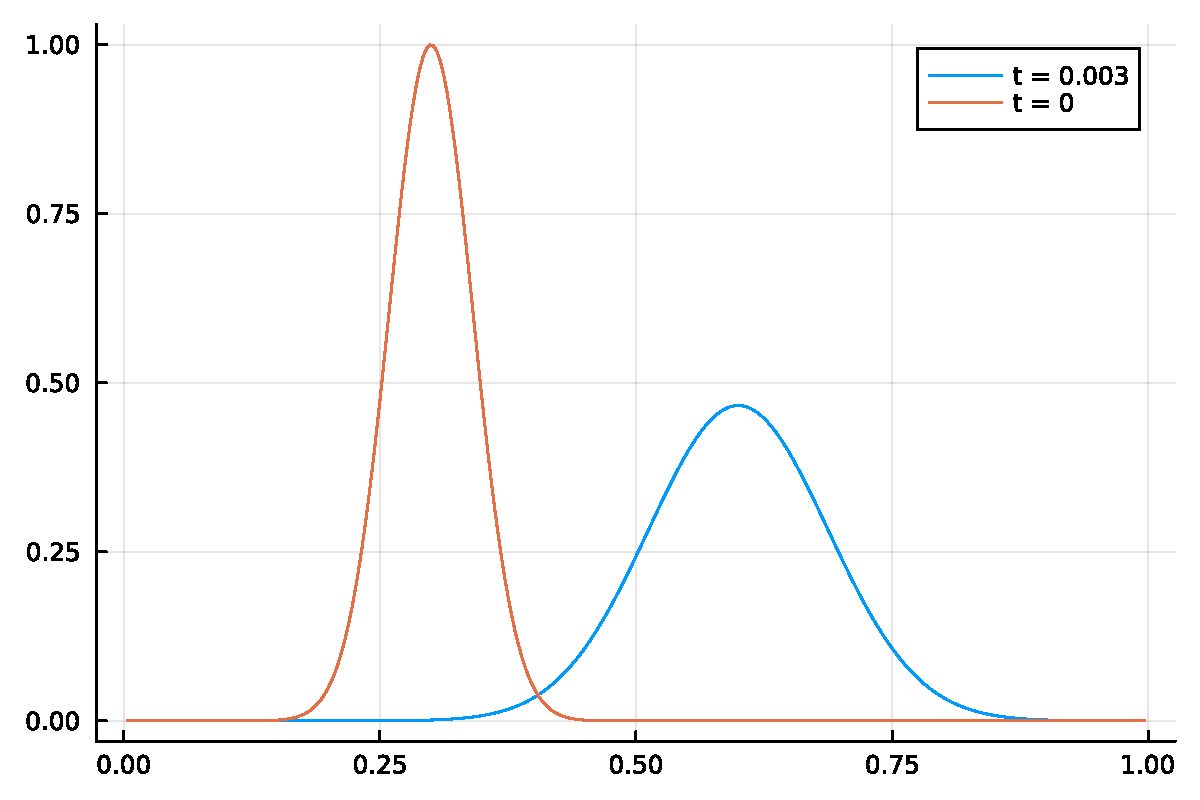
\includegraphics[width=\linewidth]{jl_nS6THr/Problem_Sheet2_Solutions_2025t_1_1.pdf}


\end{document}
